\section{TIPE TIPE DATA GEOPASIAL}
DATA RASTER DAN VEKTOR
\subsection{Pembahasan}
Data Geospasial adalah data yang memuat lokasi geografis, dimensi atau ukuran, yang mana semua nya terdapat pada permukaan bumi. Data spasial SIG mempunyai dua bagian penting yang membuatnya berbeda dari data lain, yaitu informasi lokasi dan informasi atribut. Data spasial sistem informasi geografis yang berisi informasi lokasi (informasi spasial) contohnya adalah informasi lintang dan bujur, termasuk diantaranya informasi datum dan proyeksi. Contoh lain dari informasi spasial yang bisa digunakan untuk mengidentifikasikan lokasi misalnya adalah Kode Pos. Sedangkan Informasi Atribut (deskriptif) biasa disebut juga dengan informasi non-spasial. Suatu lokalitas bisa mempunyai beberapa atribut atau properti yang berkaitan dengannya; contohnya jenis vegetasi, populasi, pendapatan per tahun, dan lain-lain.Data geospasial dibagi mejadi dua tipe jenis, diantaranya:

\begin{enumerate}
\item Data vektor adalah data yang direpresentasikan sebagai suatu mosaik berupa garis (arc/\textit{line}), polygon (daerah yang dibatasi oleh garis yang berawal dan berakhir pada titik yang sama), titik/\textit{point} (node yang mempunyai label), dan \textit{nodes} (merupakan titik perpotongan antara dua buah garis). Keuntungan utama dari format data vektor adalah ketepatan dalam merepresentasikan fitur titik, batasan dan garis lurus. Kegunaan Data Vektor untuk analisa yang membutuhkan ketepatan posisi, misalnya pada basis data batas-batas kadaster. Contoh penggunaan lainnya adalah untuk mendefinisikan hubungan spasial dari beberapa fitur. Kelemahan data vektor yang utama adalah ketidakmampuannya dalam mengakomodasi perubahan gradual. Data vektor ini disimpan dalam file ber ekstensi .shp atau shapefile esri.
	\begin{enumerate}
	\item \textit{LINE}/\textit{PATH}
	\item \textit{POLYGON}
	\item \textit{POINT}
	\end{enumerate}
		\begin{figure}[htbp]
		\centering
		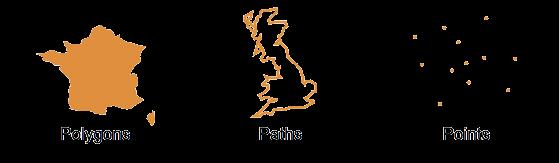
\includegraphics[width=0.75\textwidth]{pictures/datavektor.jpg}
		\caption{salah satu contoh gambar data vektor}
		\label{labelgambar1}
		\end{figure}	
	Pada gambar 1 terlihat 3 bentuk data jenis vector yaitu \textit{polygon} yang berbentuk wilayah, \textit{path} yang berbentuk garis dan point yang berbentuk titik titik.
\item Data raster adalah data yang dihasilkan dari penginderaan jauh. Data Raster sering disebut juga dengan sel grid. Pada data raster, obyek geografis direpresentasikan sebagai struktur sel grid yang disebut dengan pixel (\textit{picture element}). Pada data raster, resolusi (definisi visual) tergantung pada ukuran pixel-nya. Dengan kata lain, resolusi pixel menggambarkan ukuran sebenarnya di permukaan bumi yang diwakili oleh setiap pixel pada citra.
Semakin kecil ukuran permukaan bumi yang direpresentasikan oleh satu sel, semakin tinggi resolusinya. Data raster sangat baik untuk merepresentasikan batas-batas yang berubah secara gradual, seperti jenis tanah, kelembaban tanah, vegetasi, suhu tanah, dan sebagainya. Kelemahan utama dari data raster adalah besarnya ukuran file; semakin tinggi resolusi grid-nya semakin besar pula ukuran filenya.
\end{enumerate}



